\begin{figure}[p]
    \thispagestyle{empty}
    \centering
    \rotatebox{90}{
        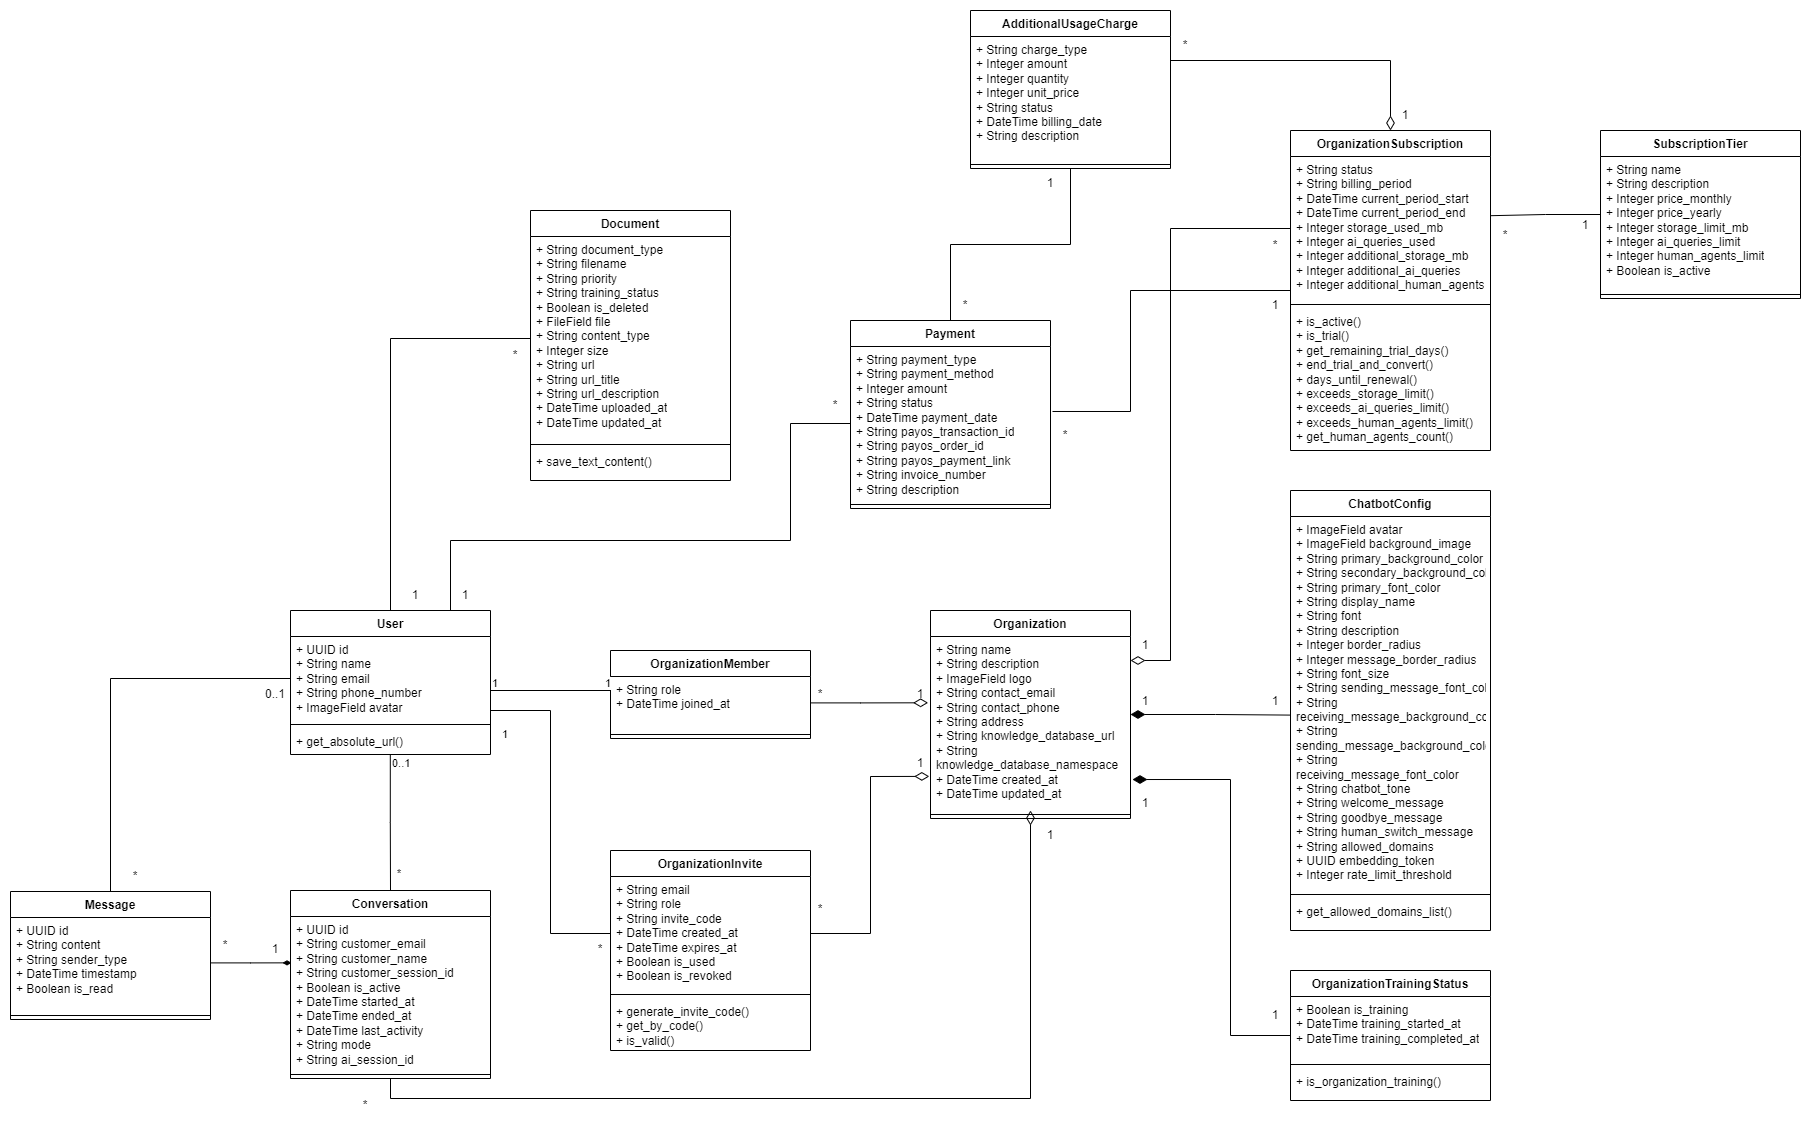
\includegraphics[height=0.9\textwidth, width=0.9\textheight, keepaspectratio]{Dg_Class/class.png}
    }
    \rotatebox{90}{
        \parbox{\textwidth}{
            \centering
            \caption{Biểu đồ class các thực thể cho tầng dữ liệu}
            \label{fig:enter-label}
        }
    }
\end{figure}


\begin{itemize}[leftmargin=*, labelsep=5mm] % Adjust margins if needed

    % ========================================
    \item \textbf{Quản lý Người dùng (User Management)}
    % ========================================
    \begin{itemize}[leftmargin=*, labelsep=4mm]
        \item \textbf{User}
        \begin{itemize}[leftmargin=*, labelsep=3mm]
            \item \textit{Mục đích}: Quản lý các thông tin định danh và cơ bản của người dùng hệ thống.
            \item \textit{Thuộc tính chính}: \texttt{id}, \texttt{name}, \texttt{email}, \texttt{phone\_number}, \texttt{avatar}.
            \item \textit{Quan hệ (Relationships)}:
            \begin{itemize}[leftmargin=*, labelsep=2mm]
                \item Liên kết đơn nhất tới một thực thể \texttt{OrganizationMember}.
                \item Có thể đóng vai trò nhân viên hỗ trợ tham gia vào nhiều thực thể \texttt{Conversation}.
                \item Là người khởi tạo của nhiều thực thể \texttt{Message}.
                \item Là người khởi tạo nhiều thực thể \texttt{OrganizationInvite}.
                \item Là người tải lên của nhiều thực thể \texttt{Document}.
                \item Là người khởi tạo nhiều giao dịch \texttt{Payment}.
            \end{itemize}
            \item \textit{Chức năng chính}: Lưu trữ và quản lý thông tin định danh của người dùng.
        \end{itemize}
    \end{itemize}

    % ========================================
    \item \textbf{Quản lý Tổ chức (Organization Management)}
    % ========================================
    \begin{itemize}[leftmargin=*, labelsep=4mm]
        \item \textbf{Organization}
        \begin{itemize}[leftmargin=*, labelsep=3mm]
            \item \textit{Mục đích}: Quản lý thông tin, cấu hình và các tài nguyên liên quan đến một tổ chức sử dụng hệ thống.
            \item \textit{Thuộc tính chính}: \texttt{name}, \texttt{description}, \texttt{logo}, \texttt{contact\_email}, \texttt{contact\_phone}, \texttt{address}, \texttt{knowledge\_database\_url}, \texttt{knowledge\_database\_namespace}, \texttt{created\_at}, \texttt{updated\_at}.
            \item \textit{Quan hệ (Relationships)}:
            \begin{itemize}[leftmargin=*, labelsep=2mm]
                \item Bao gồm nhiều thành viên thông qua thực thể \texttt{OrganizationMember}.
                \item Quản lý nhiều lời mời tham gia thông qua thực thể \texttt{OrganizationInvite}.
                \item Liên kết đơn nhất tới một cấu hình chatbot (\texttt{ChatbotConfig}).
                \item Bao gồm nhiều tài liệu huấn luyện (\texttt{Document}).
                \item Liên kết đơn nhất tới một trạng thái huấn luyện (\texttt{OrganizationTrainingStatus}).
                \item Quản lý nhiều gói đăng ký dịch vụ thông qua thực thể \texttt{OrganizationSubscription}.
                \item Bao gồm nhiều cuộc hội thoại (\texttt{Conversation}).
                \item Quản lý nhiều giao dịch thanh toán (\texttt{Payment}).
            \end{itemize}
            \item \textit{Chức năng chính}: Đóng vai trò trung tâm quản lý thông tin, cấu hình và tài nguyên liên quan đến tổ chức.
        \end{itemize}

        \item \textbf{OrganizationMember}
        \begin{itemize}[leftmargin=*, labelsep=3mm]
            \item \textit{Mục đích}: Quản lý vai trò và thông tin tham gia của một người dùng cụ thể trong tổ chức.
            \item \textit{Thuộc tính chính}: \texttt{role} [OWNER, ADMIN, AGENT], \texttt{joined\_at}.
            \item \textit{Quan hệ (Relationships)}:
            \begin{itemize}[leftmargin=*, labelsep=2mm]
                \item Liên kết đơn nhất tới một thực thể \texttt{User}.
                \item Thuộc về một thực thể \texttt{Organization} duy nhất.
            \end{itemize}
            \item \textit{Chức năng chính}: Xác định vai trò của thành viên và ghi nhận thời điểm bắt đầu tham gia tổ chức.
        \end{itemize}

        \item \textbf{OrganizationInvite}
        \begin{itemize}[leftmargin=*, labelsep=3mm]
            \item \textit{Mục đích}: Quản lý các lời mời dành cho người dùng mới tham gia vào tổ chức.
            \item \textit{Thuộc tính chính}: \texttt{email}, \texttt{role}, \texttt{invite\_code}, \texttt{created\_at}, \texttt{expires\_at}, \texttt{is\_used}, \texttt{is\_revoked}.
            \item \textit{Quan hệ (Relationships)}:
            \begin{itemize}[leftmargin=*, labelsep=2mm]
                \item Thuộc về một thực thể \texttt{Organization} duy nhất.
                \item Được tạo bởi một \texttt{User} (người mời).
            \end{itemize}
            \item \textit{Chức năng chính}: Cung cấp các chức năng tạo mã mời, truy xuất lời mời theo mã, và kiểm tra tính hợp lệ của lời mời.
        \end{itemize}
    \end{itemize}

    % ========================================
    \item \textbf{Quản lý Gói cước \& Thanh toán (Subscription \& Billing)}
    % ========================================
    \begin{itemize}[leftmargin=*, labelsep=4mm]
        \item \textbf{SubscriptionTier}
        \begin{itemize}[leftmargin=*, labelsep=3mm]
            \item \textit{Mục đích}: Định nghĩa các cấp độ gói dịch vụ, bao gồm các giới hạn tài nguyên và chi phí tương ứng.
            \item \textit{Thuộc tính chính}: \texttt{name} [FREE, STARTER, PROFESSIONAL], \texttt{description}, \texttt{price\_monthly}, \texttt{price\_yearly}, \texttt{storage\_limit\_mb}, \texttt{ai\_queries\_limit}, \texttt{human\_agents\_limit}, \texttt{is\_active}.
            \item \textit{Quan hệ (Relationships)}:
            \begin{itemize}[leftmargin=*, labelsep=2mm]
                \item Là cơ sở định nghĩa cho nhiều thực thể \texttt{OrganizationSubscription}.
            \end{itemize}
            \item \textit{Chức năng chính}: Cung cấp thông tin chi tiết về các gói dịch vụ khả dụng.
        \end{itemize}

        \item \textbf{OrganizationSubscription}
        \begin{itemize}[leftmargin=*, labelsep=3mm]
            \item \textit{Mục đích}: Quản lý gói dịch vụ hiện tại của một tổ chức, bao gồm trạng thái, chu kỳ thanh toán và mức độ sử dụng tài nguyên.
            \item \textit{Thuộc tính chính}: \texttt{status}, \texttt{billing\_period}, \texttt{current\_period\_start}, \texttt{current\_period\_end}, \texttt{storage\_used\_mb}, \texttt{ai\_queries\_used}, \texttt{additional\_storage\_mb}, \texttt{additional\_ai\_queries}, \texttt{additional\_human\_agents}.
            \item \textit{Quan hệ (Relationships)}:
            \begin{itemize}[leftmargin=*, labelsep=2mm]
                \item Thuộc về một thực thể \texttt{Organization} duy nhất.
                \item Liên kết đơn nhất tới một thực thể \texttt{SubscriptionTier}.
                \item Liên quan đến nhiều thực thể phí phát sinh (\texttt{AdditionalUsageCharge}).
                \item Liên quan đến nhiều giao dịch thanh toán (\texttt{Payment}).
            \end{itemize}
            \item \textit{Chức năng chính}: Quản lý trạng thái đăng ký, xử lý gia hạn, kiểm tra giới hạn sử dụng và theo dõi tài nguyên đã tiêu thụ.
        \end{itemize}

        \item \textbf{AdditionalUsageCharge}
        \begin{itemize}[leftmargin=*, labelsep=3mm]
            \item \textit{Mục đích}: Ghi nhận các khoản phí phát sinh từ việc sử dụng tài nguyên vượt mức hoặc mua thêm tài nguyên bổ sung.
            \item \textit{Thuộc tính chính}: \texttt{charge\_type}, \texttt{amount}, \texttt{quantity}, \texttt{unit\_price}, \texttt{status}, \texttt{billing\_date}, \texttt{description}.
            \item \textit{Quan hệ (Relationships)}:
            \begin{itemize}[leftmargin=*, labelsep=2mm]
                \item Liên kết tới một thực thể \texttt{OrganizationSubscription}.
                \item Liên quan đến một hoặc nhiều giao dịch thanh toán (\texttt{Payment}).
                \item Thuộc về một thực thể \texttt{Organization} (thông qua \texttt{OrganizationSubscription}).
            \end{itemize}
            \item \textit{Chức năng chính}: Ghi nhận chi tiết các khoản phí phát sinh, phục vụ cho việc tạo hóa đơn.
        \end{itemize}

        \item \textbf{Payment}
        \begin{itemize}[leftmargin=*, labelsep=3mm]
            \item \textit{Mục đích}: Ghi nhận thông tin chi tiết về các giao dịch thanh toán được thực hiện.
            \item \textit{Thuộc tính chính}: \texttt{payment\_type}, \texttt{payment\_method}, \texttt{amount}, \texttt{status}, \texttt{payment\_date}, \texttt{payos\_transaction\_id}, \texttt{payos\_order\_id}, \texttt{payos\_payment\_link}, \texttt{invoice\_number}, \texttt{description}.
            \item \textit{Quan hệ (Relationships)}:
            \begin{itemize}[leftmargin=*, labelsep=2mm]
                \item Thuộc về một thực thể \texttt{Organization} duy nhất.
                \item Có thể được khởi tạo bởi một \texttt{User}.
                \item Liên quan đến một thực thể \texttt{OrganizationSubscription}.
                \item Liên quan đến một hoặc nhiều bản ghi \texttt{AdditionalUsageCharge}.
            \end{itemize}
            \item \textit{Chức năng chính}: Lưu trữ lịch sử giao dịch và theo dõi trạng thái hoàn thành của các khoản thanh toán.
        \end{itemize}
    \end{itemize}

    % ========================================
    \item \textbf{Cấu hình Chatbot \& AI (Chatbot \& AI Configuration)}
    % ========================================
    \begin{itemize}[leftmargin=*, labelsep=4mm]
        \item \textbf{ChatbotConfig}
        \begin{itemize}[leftmargin=*, labelsep=3mm]
            \item \textit{Mục đích}: Lưu trữ các thiết lập liên quan đến giao diện hiển thị và hành vi hoạt động của chatbot.
            \item \textit{Thuộc tính chính}: \texttt{avatar}, \texttt{background\_image}, \texttt{colors}, \texttt{fonts}, \texttt{display\_name}, \texttt{messages}, \texttt{allowed\_domains}, \texttt{embedding\_token}, \texttt{rate\_limit\_threshold}. % Removed "etc."
            \item \textit{Quan hệ (Relationships)}:
            \begin{itemize}[leftmargin=*, labelsep=2mm]
                \item Thuộc về một thực thể \texttt{Organization} duy nhất.
            \end{itemize}
            \item \textit{Chức năng chính}: Cho phép tùy chỉnh giao diện và hành vi chatbot, quản lý danh sách tên miền được phép nhúng, và hỗ trợ kiểm soát truy cập.
        \end{itemize}

        \item \textbf{Document}
        \begin{itemize}[leftmargin=*, labelsep=3mm]
            \item \textit{Mục đích}: Quản lý các tài liệu được sử dụng làm cơ sở tri thức để huấn luyện mô hình AI của chatbot.
            \item \textit{Thuộc tính chính}: \texttt{document\_type} [FILE, TEXT, URL], \texttt{filename}, \texttt{priority}, \texttt{training\_status}, \texttt{is\_deleted}, \texttt{file}, \texttt{content\_type}, \texttt{size}, \texttt{url}, \texttt{url\_title}, \texttt{url\_description}, \texttt{uploaded\_at}, \texttt{updated\_at}.
            \item \textit{Quan hệ (Relationships)}:
            \begin{itemize}[leftmargin=*, labelsep=2mm]
                \item Thuộc về một thực thể \texttt{Organization} duy nhất.
                \item Được tải lên bởi một \texttt{User} (người tải lên).
            \end{itemize}
            \item \textit{Chức năng chính}: Lưu trữ tài liệu huấn luyện, quản lý trạng thái xử lý, và thực hiện các tác vụ liên quan đến nội dung.
        \end{itemize}

        \item \textbf{OrganizationTrainingStatus}
        \begin{itemize}[leftmargin=*, labelsep=3mm]
            \item \textit{Mục đích}: Theo dõi trạng thái quá trình huấn luyện mô hình AI dựa trên cơ sở tri thức của toàn bộ tổ chức.
            \item \textit{Thuộc tính chính}: \texttt{is\_training}, \texttt{training\_started\_at}, \texttt{training\_completed\_at}.
            \item \textit{Quan hệ (Relationships)}:
            \begin{itemize}[leftmargin=*, labelsep=2mm]
                \item Thuộc về một thực thể \texttt{Organization} duy nhất.
            \end{itemize}
            \item \textit{Chức năng chính}: Cung cấp thông tin về trạng thái huấn luyện hiện tại và ghi nhận lịch sử các lần huấn luyện đã hoàn thành.
        \end{itemize}
    \end{itemize}

    % ========================================
    \item \textbf{Quản lý Hội thoại (Conversation Management)}
    % ========================================
    \begin{itemize}[leftmargin=*, labelsep=4mm]
        \item \textbf{Conversation}
        \begin{itemize}[leftmargin=*, labelsep=3mm]
            \item \textit{Mục đích}: Đại diện và quản lý một phiên hội thoại hoàn chỉnh giữa khách hàng cuối và hệ thống chatbot hoặc nhân viên hỗ trợ.
            \item \textit{Thuộc tính chính}: \texttt{id}, \texttt{customer\_email}, \texttt{customer\_name}, \texttt{customer\_session\_id}, \texttt{is\_active}, \texttt{started\_at}, \texttt{ended\_at}, \texttt{last\_activity}, \texttt{mode}, \texttt{ai\_session\_id}.
            \item \textit{Quan hệ (Relationships)}:
            \begin{itemize}[leftmargin=*, labelsep=2mm]
                \item Bao gồm một chuỗi các thực thể \texttt{Message} thể hiện nội dung trao đổi.
                \item Thuộc về một thực thể \texttt{Organization} duy nhất.
                \item Có thể được tiếp nhận và xử lý bởi một \texttt{User} đóng vai trò nhân viên hỗ trợ (agent).
            \end{itemize}
            \item \textit{Chức năng chính}: Lưu trữ thông tin định danh khách hàng, toàn bộ lịch sử tin nhắn, và quản lý trạng thái của cuộc hội thoại.
        \end{itemize}

        \item \textbf{Message}
        \begin{itemize}[leftmargin=*, labelsep=3mm]
            \item \textit{Mục đích}: Đại diện cho một tin nhắn trao đổi trong một cuộc hội thoại.
            \item \textit{Thuộc tính chính}: \texttt{id}, \texttt{content}, \texttt{sender\_type} [CUSTOMER, AGENT, AI, SYSTEM], \texttt{timestamp}, \texttt{is\_read}.
            \item \textit{Quan hệ (Relationships)}:
            \begin{itemize}[leftmargin=*, labelsep=2mm]
                \item Thuộc về một thực thể \texttt{Conversation} duy nhất.
                \item Có thể được gửi bởi một \texttt{User} (khách hàng hoặc nhân viên hỗ trợ), hoặc được tạo bởi AI hoặc hệ thống.
            \end{itemize}
            \item \textit{Chức năng chính}: Lưu trữ nội dung tin nhắn, thông tin người gửi (khách hàng, nhân viên hỗ trợ, AI, hệ thống) và thời gian.
        \end{itemize}
    \end{itemize}

\end{itemize}
